
\title{Recap Computer System Security (02KRQOV)}
\author{Jacopo Nasi\\
        Computer Engineer\\
        Politecnico di Torino}
\date{I Period - 2018/2019\\\bigskip\bigskip\today}

\documentclass[12pt]{article}
\usepackage[utf8]{inputenc}
\usepackage[english]{babel}
\usepackage{geometry}
\usepackage{indentfirst} % First line indent
\usepackage{mathtools}
\usepackage{wrapfig}
\usepackage[usenames, dvipsnames]{color}
\usepackage{float}
\usepackage{amssymb}
\usepackage{ifsym}
\usepackage{listings}
\usepackage{multicol}

% Misure Documento
\geometry{ a4paper, total={170mm,257mm},left=35mm, right=35mm, top=35mm, bottom=35mm }

\begin{document}

\begin{figure}
  \centering
  
\includegraphics[width=10cm]{images/polito.pdf}
\end{figure}

\maketitle


\newpage
\tableofcontents

\newpage
{\noindent \Large \textbf{License}\bigskip}

This work is licensed under a Creative Commons Attribution-NonCommercial-ShareAlike 3.0 Unported License.\\
You are free:
\begin{itemize}
  \item \textbf{to Share}: to copy, distribute and transmit the work
  \item \textbf{to Remix}: to adapt the work
\end{itemize}
Under the following conditions:
\begin{itemize}
  \item \textbf{Attribution}: you must attribute the work in the manner specified by the author or licensor (but not in any way that suggests that they endorse you or your use of the work)
  \item \textbf{Noncommercial}: you may not use this work for commercial purposes.
  \item \textbf{Share Alike}: if you alter, transform, or build upon this work, you may distribute the resulting work only under the same or similar license to this one.
\end{itemize}

\noindent More information on the Creative Commons website (http://creativecommons.org).

\begin{figure}[h!]
  \centering
  
\includegraphics[width=3cm]{images/license.png}
\end{figure}

{\noindent \Large \textbf{Acknowledgments}\bigskip}

Questo breve riepilogo non ha alcuno scopo se non quello di agevolare lo studio di me stesso, se vi fosse di aiuto siete liberi di usarlo.\\
Le fonti su cui mi sono basato sono quelle relative al corso offerto (\textbf{Computer System Security (02KRQOV)}) dal Politecnico di Torino durante l'anno accademico 2018/2019.\\
Non mi assumo nessuna responsabilità in merito ad errori o qualsiasi altra cosa. Fatene buon uso!
\newpage

\section{Introduction Security ICT System}
\textbf{Why is securoty an important issue?} Nowadays that everything is online and connected to a world wild network, the security over the ICT system has become fundamental. A lack of the secutiry could generate lose for milions of money. Also data breach become a problem.\\
Everydays technology improve and drive innovation but security must be improved together with the innovations.\\
With the increase of the number of connected devices, the IoT (Internet of Things), security start to facing a lot of more problem, the complexity of the scenario has become really really big. From personal devices, like desktop, laptop, fridge or car, by communications networks, and to distributed services, everything must be secured!\\
\paragraph{Complexity enemy of security} based on one of the first axiom of engineering: \textit{"The more complex a syste, is, the more difficult its correctness verification will be."}. Keep a system as simple as possible is always a good idea. The KISS rules (\textbf{\textit{Keep It Simple, Stupid}}) is one of the most important rule over the system security.
\paragraph{Definition of ICT Security}

\bigskip
``It is the set of products, services, organization rules and individual behaviours that protect the ICT system of a company.\\

It has the duty to protect the resources from undesired access, guarantee the privacy of information, ensure the service operation and availability in case of unpredictable events (C.I.A. = Confidentiality, Integrity, Availability).\\

The objective is to guard the information with the same professionalism and attention as for the jewels and deposit certificates stored in a bank caveau.\\

The ICT system is the safe of our most valuable information; ICT security is the equivalent of the locks, combinations and keys required to protect it.''\\
\rightline{{\rm --- \textbf{Italian Bank}}}
\bigskip

An important part of the security study is the Risk Estimation, is a fundamental step that take in account all the assets and events to evaluate the risk of something. The flow is showed in figure \ref{fig:risk_est}:

\begin{figure}[h!]
  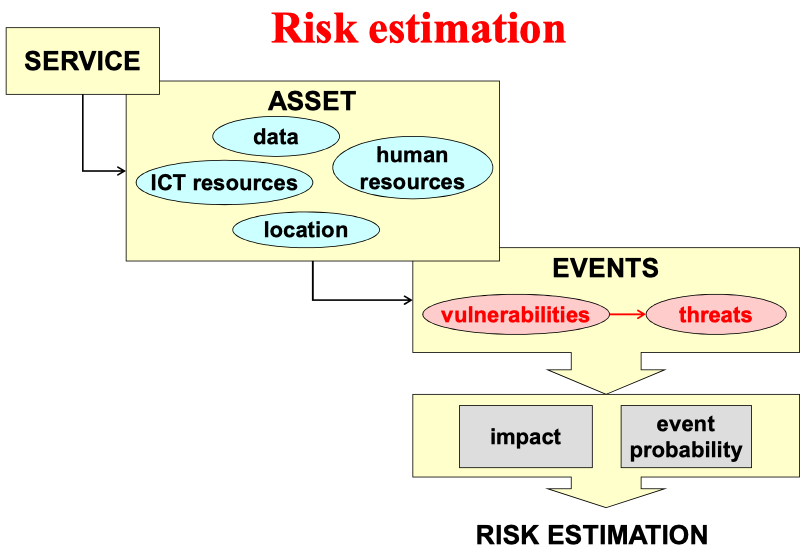
\includegraphics[width=\linewidth]{images/risk_est.png}
  \caption{Risk Estimation}
  \label{fig:risk_est}
\end{figure}

Where the assets is composed by everythings needed by a service to work, both soft and hard part, also human resources. The vulnerabilities, intrinsic of an asset, represent the weakness of it. The threats is a deliberate action, or an accidental event, that can produce the loss of a security properties exploting a vulnerability. The event is also characterized by an impact and a probability that could be high, low or other middle values.\\
Direct following of the risk estimation is the Analysis and management of security. After the evaluation of risks, is necessary to:
\begin{enumerate}
  \item Select Countermeasures
  \item Implement Countermeasures
  \item Audit (check if works)
\end{enumerate}

The security implement is not a phase of the developmente process, is part of each sigle part of it. Security can't be compute at the end of the development, it must be implement from the beginning of the process. \textbf{Security is a process, not a product!} The following figure \ref{fig:dev} show the parallel line followed by the security development.

\begin{figure}[h!]
  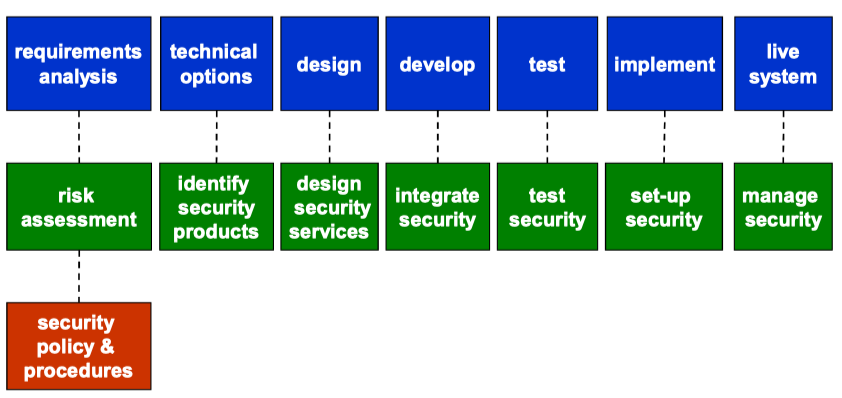
\includegraphics[width=\linewidth]{images/dev.png}
  \caption{Security Life Cycle}
  \label{fig:dev}
\end{figure}

An important definition, before speaking about security itself, is the \textbf{Window of Exposure} the represent the time when an attack could be perfomed and there are no countermeasures to avoid it. This window could potentially be infinite and this is the real problem.
The figure \ref{fig:window} show how this windows id divided in different part:

\begin{figure}[h!]
  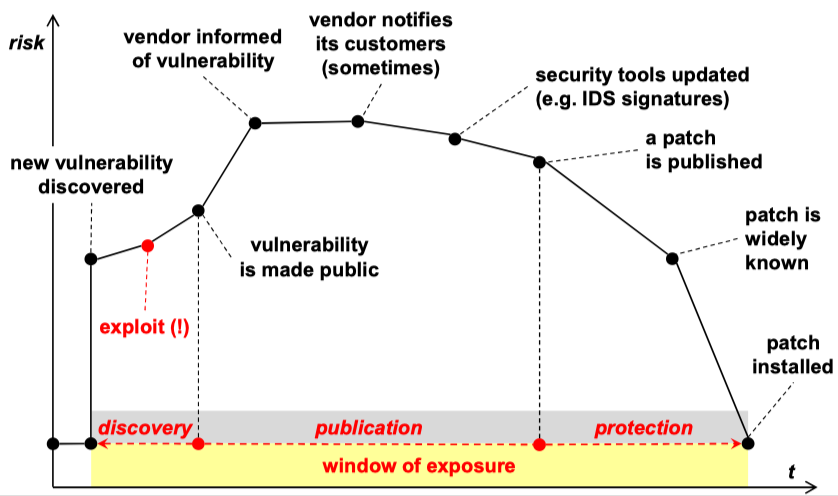
\includegraphics[width=\linewidth]{images/window.png}
  \caption{Window of Exposure}
  \label{fig:window}
\end{figure}

As already says, security is not a product but is a proccess. Computer flaws are inevitable and this is way we can't use devote our security to only secured products. The only way to effectively do business is an insecure world is to put processes in place that recognize the inheritent insecurity in the products. \textbf{The trick is to reduce your risk of exposure regardless of the products or patches}.
























\end{document}
